\label{chapter:conceitos}
\par
Este capítulo tem como objetivo apresentar os principais conceitos e definições abordados neste trabalho, tais como: Knowledge Discovery in Database (KDD), Mineração de dados, Aprendizagem de Máquina e Mineração de Dados Educacionais.

%============================
% KDD
%============================
\section{Knowledge Discovery in Database (KDD)}

A palvra KDD, sigla de \textit{Knowledge Discovery in Database} que em português é descoberta de conhecimento em bases de dados, foi formalizado em 1989, com intuito de atender os processos referente a busca e extração do conhecimento a partir de bases de dados \cite{Isamir2010}. Segundo \citeonline{Fayyad1996}, KDD é um método formado de várias etapas, não trivial, interativo e iterativo, para o reconhecimento de padrões passível de compreensão, relevantes, novos e potencialmente úteis a partir de grandes grupos de dados.

\par
Considerando a importância de cada componente: \textbf{metódo} se refere a um conjunto de técnicas sequenciais para se conseguir o conhecimento a partir dos dados. \textbf{Padrões} indica unidades que se repetem de maneira previsível. \textbf{Relevante} que tem grau de importância para os padrões descobertos. \textbf{Novos} refere-se as informações não conhecidas sobre os dados, obtidas através dos padrões encontrados. \textbf{Compreensão} indica o nível de entendimento do contexto da solução, que esse padrão pode oferecer aos que utilizarão o conhecimento \cite{Marques2014}.

\par
Segundo \cite{Isamir2010} o processo de KDD extraí e deriva o conhecimento útil dos padrões de dados, que se relacionam por tarefas funcionais, podendo assim, ajudar nas tomadas de decisão. É importante saber que o interativo indica a atuação humana sobre o KDD, no sentido de ele ser o responsável de analisar e interpretar dados e padrões, e o iterativo indica a necessidade de inúmeras vezes a repetição do processo de forma integral e parcial para se obter um resultado satisfatório.

\par
O processo de KDD é constituído por etapas ou fases operacionais organizadas em sequência, como pode ser mostrado na Figura 1:

\begin{itemize}
    \item \textbf{Seleção:} Essa etapa está relacionada a estudar os dados que são disponíveis na base e sua importância, na tentativa de buscar soluções para os problemas identificados \cite{Kampff2013}.
    \item \textbf{Pré-Processamento:} Após da etapa inicial, vem a parte de pré-processamento que tem como objetivo de garantir a qualidade dos dados que estão incluídos no KDD, realizando assim operações básicas como a remoção de ruídos \cite{Dantas2008}.
    \item \textbf{Transformação:} Esta etapa consiste na seleção e transformação dos dados no formato apropriado aos algoritmos e ferramentas de mineração utilizados, como por exemplo em arquivos CSV (\textit{Comma-Separated Values}) \cite{Kampff2013}.
    \item \textbf{Mineração de Dados:} Depois da realização das etapas anteriores, a mineração de dados é iniciada. Ela se constitui na principal etapa do KDD, pois, através dela que as informações ocultas e potencialmente importantes serão extraídas \cite{Kampff2013}. 
    \item \textbf{Pós-Processamento:} Após a mineração de dados começa a avaliação dos resultados, que praticamente envolve a identificação do conhecimento que foi extraído na busca de padrões interessantes, que será utilizado para ajudar na solução dos problemas que incentivaram a mineração \cite{Dantas2008}.
\end{itemize}

\begin{figure}[!htp]
	\begin{center}
    \caption{\label{fig:waveform_fig}Etapas para descoberta de conhecimento adaptada de \cite{Fayyad1996}.}
	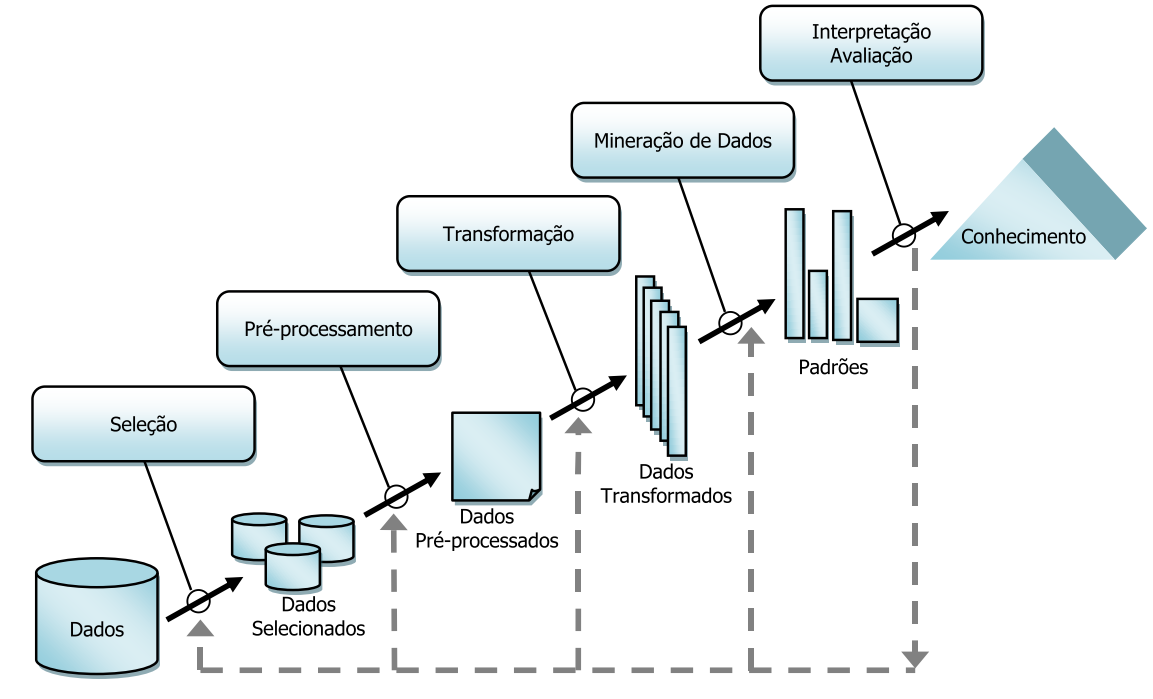
\includegraphics[scale=0.55]{Figuras/Etapas_KDD.png}
	\end{center}
    \legend{Fonte:\cite{Kampff2013}}
\end{figure}

\par
Por tanto ao termino da avaliação, o conhecimento extraído na mineração será introduzido e incorporado por outros sistemas, documentando e disponibilizando os métodos, afim  de apresentar o conhecimento obtido ao usuário ou, mais importante de servir como suporte para a tomada de decisão \cite{Kampff2013}. Resumidamente, essas cinco etapas do processo de KDD podem ser classificadas em três categorias: pré-processamento, mineração de dados e pós-processamento, como é apresentado na Figura 2 \cite{Fayyad1996}.

\begin{figure}[!htp]
	\begin{center}
    \caption{\label{fig:waveform_fig}As três partes da divisão do KDD segundo \cite{Fayyad1996}.}
	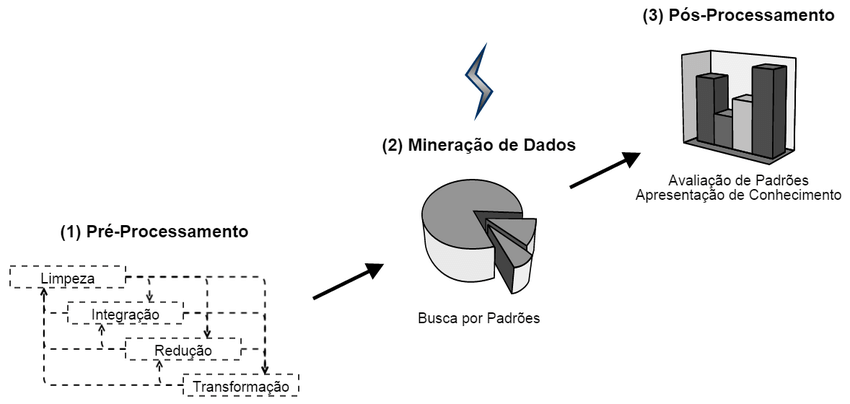
\includegraphics[scale=0.55]{Figuras/Tres_partes_KDD.png}
	\end{center}
    \legend{Fonte:\cite{Maciel}}
\end{figure}

\par
Como vimos antes, a aplicação de KDD, especificamente na etapa de mineração de dados, podemos perceber a sua enorme importância para todas as áreas que necessitem retirar informações de uma base forte e concreta de dados. Com isso, para a próxima seção, serão apresentados os conceitos relacionado a mineração de dados onde será aprofundado mais sobre essa fase explicando sua metodologia e tarefas de mineração.



%==========================
% MINERAÇÃO DE DADOS
%==========================

\section{Mineração de Dados}

O termo Mineração de dados (MD, do inglês, \textit{Data Mining}, DM), conhecido tambem como uma etapa do KDD, pertence a disciplina que tem como objetivo de encontrar novas informações através da análise de grandes volumes de dados. No caso a frase \textbf{novas informações} está se referindo ao processo de reconhecer novos conhecimentos, assim gerando mais descobertas científicas \cite{Baker2011}.

\par
Segundo \citeonline{Amaral2016}, a mineração de dados seria vários processos para explorar e analisar grandes quantidades de dados na busca de padrões, previsões, erros, associações e entre outros. Em outras palavras, as ferramentas de MD examinam os dados, descobrem oportunidades escondidas ou problemas nos relacionamentos dos dados, e então identificam o comportamento dos negócios, envolvendo a mínima interferência do usuário, fazendo com que ele só se dedique a buscar o conhecimento \cite{Jefferson}. 

\par
Comumente a mineração de dados está relacionada a aprendizagem de máquina, que na área de inteligência artificial desenvolve algoritmos capazes de fazer com o que o computador aprenda a partir do passado, isto é, ele aprende utilizando dados de eventos que já aconteceram \cite{Amaral2016}. Pode-se notar, que as ferramentas de mineração são baseados em algoritmos que formam construção de blocos de inteligência artificial, redes neurais e entre outros, que ajuda a facilitar o trabalho de empresas os auxiliando a maximizar os seus lucros \cite{Jefferson}.

\par
Antes ninguém imaginaria que as aplicações de MD seria tão difundida em diversas áreas, pois, muitas delas não possuíam um modelo de dados armazenados digitalmente \cite{Amaral2016}. Hoje existe inúmeras técnicas e tarefas de mineração de dados que vem sendo utilizados com sucesso, em áreas como \textit{marketing} por exemplo, para saber quais produtos um determinado cliente pretende comprar ou em medicina para prever qual paciente vai contrair um certa doença através do seu histórico \cite{Martinhago2005}.

\par
Além de \textit{marketing} e medicina, segundo \citeonline{Amaral2016} a mineração de dados e a aprendizagem de máquina são aplicadas em outras áreas como processamento de linguagem natural, bioinformática, reconhecimento de fala, detecção de fraude,  finanças, sistemas de recomendação, robóticas, mineração de textos, educação e entre outros. No caso, neste trabalho, a mineração de dados educacional será abordado o seu conceito e importância na seção mais a adiante.

\subsection{Tarefas de Mineração de Dados}

\par

As tarefas correspondem aos problemas que podem ser tratados pela mineração de dados. Dependendo do objetivo que se pretende alcançar a seleção da tarefa deve ser feita para se aplicar sobre a base de dados, existem inúmeras tarefas, mas as que são mais utilizadas pela mineração podem ser classificadas como descrição (não-supervisionado) ou predição (supervisionado) \cite{Garcia2013, Camilo2009}.

\par
Segundo \citeonline{Santos2015}, na predição a análise é feita na forma de encontrar padrões repetidos e generalizados, com a finalidade de achar informações que estão escondidos nos dados. Já na descrição, existe argumentos já formulados onde se tenta procurar respostas que confirmem ou neguem esses argumentos, assim, verificando a sua veracidade. As tarefas mais comuns delas, são: 


\subsubsection{Associação}

\par
Uma tarefa de descrição, consiste em determinar quais itens vão ser adquiridos diretamente em uma mesma transação, isto é, quanto um conjunto de atributos favorece para a presença de outro conjunto \cite{Garcia2013}. No caso se X existir alguma transação, há a possibilidade de Y existir também, pode ser apresentado na forma: SE \textit{atributo} X ENTÃO \textit{atributo} Y \cite{Camilo2009}. 

\par
Segundo \citeonline{Camilo2009}, a associação é uma das tarefas mais conhecidas pelo fato de terem tido ótimos resultados, principalmente na área de marketing com a análise de \textbf{Cesta de Vendas}, onde é identificados quais produtos são levados juntos pelo cliente. Pode-se perceber que são muito utilizado em estudos que tentam descobrir a relação entre os itens, para assim, criarem pacotes de venda ao consumidor \cite{Garcia2013}. 


\subsubsection{Classificação}

\par
Uma tarefa de predição, ela consiste em examinar uma certa característica nos dados (\textit{X}) e atribuir uma classe previamente definida (\textit{Y}), ou seja, visa identificar qual classe um determinado registro pertença, como podemos ver representada na Figura 3 \cite{Garcia2013, Kampff2013}. Exemplos disso é classificar se uma pessoa é de renda baixa, média ou alta, ou classificar se um cliente de um banco é bom ou mau pagador, assim determinando se deve conceder ou não créditos ao mesmo.

\begin{figure}[!htp]
	\begin{center}
    \caption{\label{fig:waveform_fig} Associação entre conjuntos de dados e classes.}
	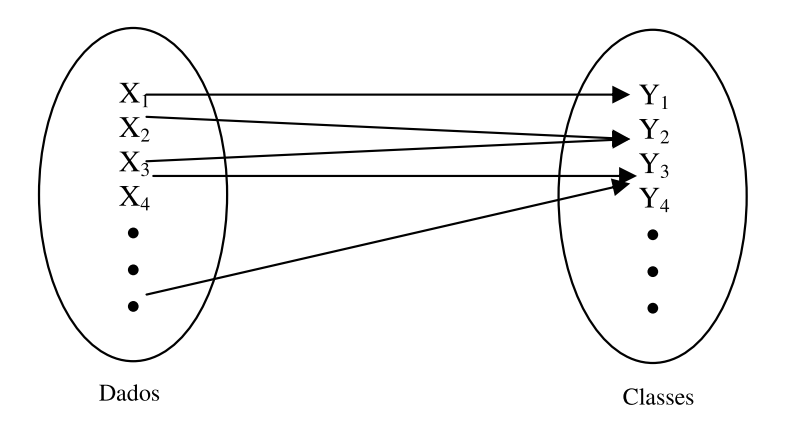
\includegraphics[scale=0.70]{Figuras/Classificacao.png}
	\end{center}
    \legend{Fonte:\cite{Rabelo2007}}
\end{figure}


\subsubsection{Regressão (Previsão ou Estimação)}

\par
Outra tarefa de predição, muito semelhante a anterior, só que com a diferença de que o atributo especial é identificado com um valor numérico e não categórico. Resume-se na estimativa do valor futuro de algum índice se baseando em dados do comportamento passado desse índice \cite{Camilo2009, LeandroSilva2014}. Exemplo, determinar se o índice da BOVESPA subirá ou descerá amanhã, prever o valor de vida de um equipamento, prever o desempenho do aluno, estimar a quantia a ser gasta por uma família de quatro pessoas durante a volta às aulas e entre outros.

\par
A técnica de regressão pode ser classificada em linear e não-linear. Segundo \citeonline{Camilo2009}, são chamados de linear quando tanto as variáveis preditivas quanto as variáveis de resposta possui um comportamento linear em sua relação, por exemplo, quando um valor Y é uma função linear de X representado na Figura 4. Já a não-linear é o oposto da linear, é quando a relação entre as variáveis de resposta e predição não segue um comportamento linear, no caso, as relações entre as variáveis podem ser representadas na forma de uma função polinomial. 

\begin{figure}[!htp]
	\begin{center}
    \caption{\label{fig:waveform_fig} Gráfico onde o valor y (pontuação alcançada) é uma função linear de x (horas de estudos).}
	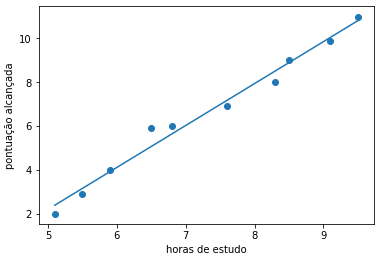
\includegraphics[scale=0.99]{Figuras/Regressao_linear.png}
	\end{center}
    \legend{Fonte:\cite{JoaoPaulo}}
\end{figure}

\subsubsection{Agrupamento (Clustering)}

\par
Outra tarefa de descrição, é um método de divisão de um conjunto de dados heterogêneos para um grupo homogêneo \cite{LeandroSilva2014}. Ele tende a reconhecer e aproximar os registros similares, isto é, ele junta um conjunto de registro semelhantes entre si que são diferentes de outros registros nos demais agrupamentos \cite{Camilo2009}. Clustering difere da classificação, pois, não necessita que os dados sejam previamente classificados (aprendizado não-supervisionado).

\par
Segundo \cite{Camilo2009}, o agrupamento não tem a intenção de predizer, estimar ou classificar uma variável, ele somente reconhece os grupos de dados iguais, como é demonstrado na Figura 5. Alguns exemplos de \textit{clustering} como agrupar clientes por região do país ou com comportamento de compra similar, agrupar alunos com desempenho semelhantes, agrupar seções de usuários Web e entre outros.


\begin{figure}[!htp]
	\begin{center}
    \caption{\label{fig:waveform_fig} Registros agrupados em três \textit{clusters}.}
	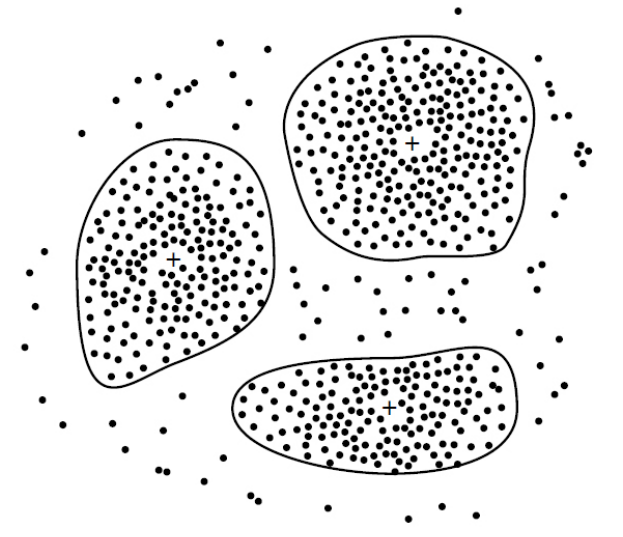
\includegraphics[scale=0.50]{Figuras/Agrupamento.png}
	\end{center}
    \legend{Fonte:\cite{Camilo2009}}
\end{figure}



\subsection{Mineração de Dados e Aprendizagem de Máquina}

\par
Como foi mencionado em tópicos anteriores, podemos perceber que a área de mineração de dados foi favorecida com diversos conceitos provenientes da área de aprendizagem de máquina, muito desses conceitos são vistos em livros voltado para essa área, tais como as técnicas de classificação, regressão, associação e agrupamento. Os dois grupos principais de mineração de dados, predição e descrição, são parecidos com a forma em que os tipos de aprendizagens são divididos: Aprendizagem supervisionada e não-supervisionada.

\par
Por tanto na próxima seção trataremos de alguns conceitos que já foram citados nesse capítulo, sendo que tais conceitos serão estudados de forma mais precisa, voltada para a área de aprendizagem de máquina.

%==========================
% APRENDIZAGEM DE MAQUINA - tecnicas(arvore de decisão, apriori...)
%==========================
\section{Aprendizagem de Máquina}

\par
Existem diversas atividades relacionadas ao conceito de aprendizagem, dificultando ainda mais a exata definição da palavra, tornando assim dependente de contexto. Porém, no contexto computacional, existe uma definição muito precisa de aprendizagem de máquina que pode ser dada \cite{Henke2011}. Segundo \citeonline{Alpaydin2009}, \textit{Machine Learning} são programas de computador que servem para melhorar um processo de um desempenho, utilizando dados de exemplo ou experiência passada.

\par
Em tese, se tem um modelo definido com alguns parâmetros, onde a aprendizagem é aplicada por um programa de computador para poder otimizar o parâmetro desse modelo utilizando dados de treinamento, sendo que, esse modelo pode ser preditivo, descritivo ou os dois \cite{Alpaydin2009}. No caso, a aprendizagem de máquina utiliza o princípio da estatística na elaboração de seus modelos, porque, a tarefa principal está fazendo a dedução a partir de uma amostra. 

\par
Segundo \citeonline{Henke2011}, os algoritmos de aprendizagem podem ser a solução para resolver diversos problemas, pois, eles podem aprender a determinar padrões das classes que estão envolvidas no problema, através de exemplos existentes obtidos do ambiente. Conforme o modelo genérico da Figura 6 sobre aprendizagem de máquina ocorre o seguinte, o ambiente concede a informação para um elemento de aprendizagem, que utiliza essa informação para melhorar a base de conhecimento para que o elemento de desempenho a use na execução de sua tarefa. 

\begin{figure}[!htp]
	\begin{center}
    \caption{\label{fig:waveform_fig} Modelo genérico de aprendizagem de máquina.}
	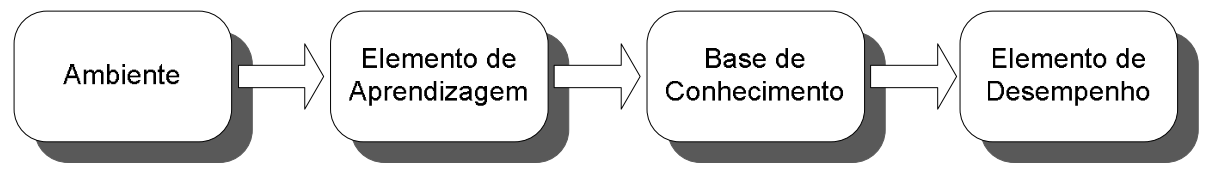
\includegraphics[scale=0.45]{Figuras/Modelo_Machine_Learning.png}
	\end{center}
    \legend{Fonte:\cite{Henke2011}}
\end{figure}

\par
Para a compreensão mais abrangente dos algoritmos de aprendizagem de máquina, é importante conhecer o conceito dos termos mais relevantes e mais usados segundo a nomenclatura abaixo de acordo com \cite{Monard2003, Souto2003, Henke2011}.

\begin{itemize}
    \item \textbf{Exemplo (padrão, instância):} É a ação ou o ato de se pegar um fato que já existe para explicar ou usar para alguma situação (por exemplo, para predição). Na maioria dos casos em aprendizagem de máquina, os exemplos são representados por vetores de características. Um exemplo uma amostra de tecido de um paciente.
    \item \textbf{Característica (atributo, variável):} É utilizado na descrição de um padrão (exemplo). Um atributo possui o seu tipo definido em um domínio, que indica os valores que ele pode apresentar (assumir). Exemplo, nível de expressão de um gene do tecido.
    \item \textbf{Vetor de características:} É quando um exemplo é descrito por uma lista de características. Um exemplo que se pode dar é um vetor m-dimensional que descreve para cada m genes, a medida do tecido de um certo paciente.
    \item \textbf{Classe:} Uma classe contém objetos parecidos, enquanto em outra classe possui objetos diferentes da dela. No caso de aprendizagem supervisionado, todo exemplo sempre possui pelo menos uma variável especial que descreve o fenômeno de interesse. Exemplo, as classes poderiam ser a presença ou a ausência de câncer no tecido.
    \item \textbf{Conjunto de exemplos (conjunto de dados):} É formado por uma quantidade de exemplos (padrões) com seus determinados valores de atributos, onde, em aprendizagem de máquina, cada exemplo é relacionado a uma classe. Geralmente, ele é dividido em dois subconjuntos separados: o conjunto de treinamento e o conjunto de teste.
    \item \textbf{Acurácia (taxa de erro):} Seria a porcentagem de erros ou acertos efetuados pelo modelo para um determinado grupo de dados. No geral, a acurácia é aplicada em testes em que em nenhum momento não foram utilizados durante o processo de aprendizagem. Existem outros meios com técnicas mais complexas na estimação da acurácia como \textit{cross-validation} e \textit{bootstrap}. 
    \item \textbf{Falso positivo:} Suponhamos que temos duas classes, A seria positivo e B negativo, o falso positivo seria a quantidade de exemplos da classe B classificados como da classe A. Já o falso negativo seria o oposto, a quantidade de exemplos A classificados como da classe B. Um exemplo bom onde ocorre isso é em matriz de confusão. 
    \item \textbf{Ruído:} Nenhum conjunto de dados é perfeito, é comum em que qualquer ambiente, acabar trabalhando com dados imperfeitos, no caso esses dados imperfeitos são conhecidos como ruído. Então, ele é definido como um conjunto de dados que aparentemente é inconsistente comparado com o restante dos dados existentes. 
    \item \textbf{\textit{Overfitting} (super-ajustamento):} É um termo que é utilizado para descrever quando um modelo se ajusta (especializa) muito bem ao conjunto de dados utilizados no seu treinamento, mas se torna ineficaz para prever novos resultados demonstrando uma taxa de acurácia baixa.
\end{itemize}

\subsection{Tipos de Aprendizagem}

\par
Segundo \citeonline{Henke2011} a aprendizagem de máquina pode ser dividido em dois tipos principais de aprendizagem: aprendizagem com professor e aprendizagem sem o professor.

\subsubsection{Aprendizagem com Professor}

\par
Conhecido também como aprendizado supervisionado, nele se tem a figura de um professor externo, no qual apresenta o conhecimento do ambiente através de um conjunto de exemplos de pares de entrada e saída, onde são propagados em uma sequência de regras que a máquina acompanhara para se obter o efeito desejado \cite{Lorena2007, Henke2011}.

\par
Exemplos desse tipo de aprendizagem, no caso de regressão, dado uma imagem de uma pessoa, através dos dados da imagem fornecido temos que prever a sua idade. Em classificação, dado um exemplo de tumor cancerígeno, temos que prever através da idade e do tamanho do tumor do paciente se ele é maligno ou benigno \cite{Pedro}.

\subsubsection{Aprendizagem sem Professor}

\par
Nesse não existe a presença de um professor, ou seja, não há exemplos rotulados de alguma função para ser aprendida \cite{Lorena2007, Henke2011}. Nessa aprendizagem são identificados dois tipos de subdivisão:

\begin{itemize}
    \item \textbf{Aprendizagem por reforço:} Não se sabe qual a saída correta. Ele se preocupa de como um agente deve agir em um ambiente de forma que potencialize alguma noção de recompensa a longo tempo. Como os pares de entrada e saída não são fornecidos, ele tenta encontrar uma maneira de mapeá-los através de uma interação contínua com o ambiente, para poder reduzir um índice escalar de desempenho \cite{Henke2011, Alpaydin2009}. 
    \item \textbf{Aprendizagem não-supervisionada:} Não existe padrões de saída desejada. O algoritmo aprende a agrupar ou representar as entradas submetidas de acordo com uma medida de qualidade. Esse tipo de aprendizagem é usada principalmente quando se quer encontrar padrões ou tendências que ajudem na compreensão dos dados, nela inclui estimação de densidade, formação de agrupamentos e dentre outros \cite{Henke2011, Lorena2007}.
\end{itemize}

\par
Exemplo de aprendizagem não-supervisionada, no caso de agrupamento, dado um determinado conjunto de 1000 pesquisas de uma universidade, queremos encontrar um jeito de agrupar automaticamente elas de acordo com suas semelhanças ou relações por diferentes variáveis, tais como frases, sequências das palavras, contagens de páginas e etc \cite{Pedro}. Já na aprendizagem por reforço, temos como exemplo jogos, robôs e navegação.


\subsection{Algoritmos de Aprendizagem}

\par
Existe uma extensa quantidade de algoritmos disponíveis para classificação/regressão em aprendizagem de máquina, sendo que serão falados apenas alguns dos principais que são mais utilizados. Todos os algoritmos que serão mencionados abaixo, podem ser utilizados tanto para classificação quanto para regressão. %\textcolor{red}{Avore de decisão - supervisionado, KNN - supervisionado, redes neurais - supervisionado, naive bayes - supervisionado, SVM - supervisionado.}


\subsubsection{Árvore de Decisão}

\par
Árvore de decisão (\textit{Decision Trees}) é uma ferramenta de aprendizagem que pode ser utilizada para tomada de decisão e dedução de valores categóricos. A ideia é de um aprendizado indutivo: se cria uma hipótese constituída em instâncias específicas que gera conclusões gerais \cite{Marques2014}. As árvores de decisão pegam como entrada um caso representado por um conjunto de atributos que retorna a uma decisão, que é a categoria para o valor de entrada


\par
Uma árvore é composta por três elementos importantes: os nós internos representam diferentes características, os ramos entre esses nós representam a possíveis valores que essas características podem possuir, enquanto os nós folhas representam o resultados, no caso, os valores de classificação da aplicação \cite{Henke2011, Barros2012}. Segundo \citeonline{Barros2012}, para a realização da classificação, deve ter uma tupla correspondente às características dos fluxos, que percorre pela árvore do nó raiz até  todos os nós folhas.  

\par
Para o melhor entendimento do processo de classificação de uma árvore de decisão, a Figura 7 mostra um exemplo usado no treinamento de dados para a tarefa de detecção de intrusão. De início, uma base de dados é fornecida ao algoritmo, onde, ele gera uma árvore feita para separar as amostras da classe Maligna de amostras da classe Benigna. Depois da construção da árvore, os dados novos podem ser fornecidos ao classificador, ao qual concedera uma das duas classes à amostra testada \cite{Henke2011}. 

\begin{figure}[!htp]
	\begin{center}
    \caption{\label{fig:waveform_fig} Treinamento dos dados em uma Árvore de Decisão.}
	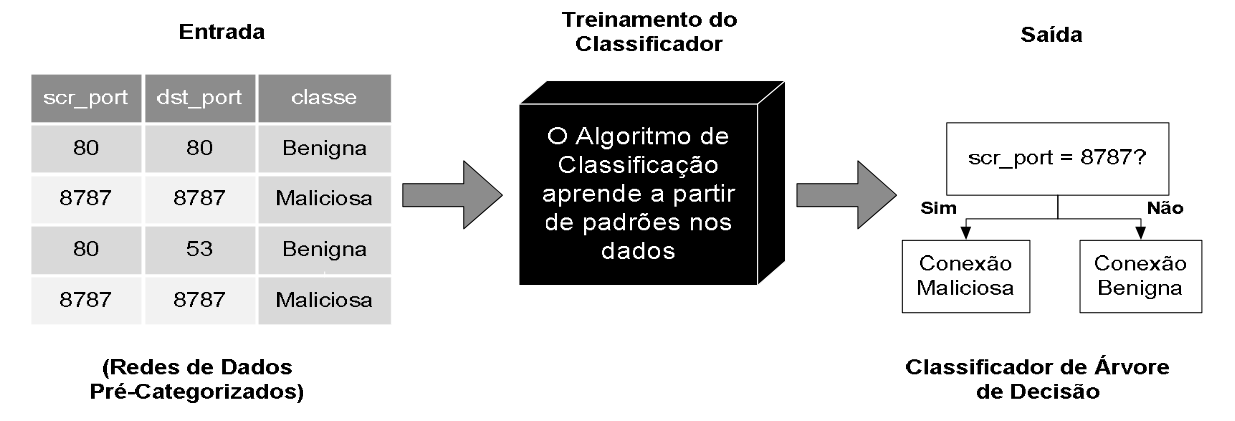
\includegraphics[scale=0.50]{Figuras/Arvore_decisao.png}
	\end{center}
    \legend{Fonte:\cite{Henke2011}}
\end{figure}

\par
Pelo que podemos perceber em um ponto de vista de decisão de negócios, uma árvore de decisão é uma quantidade mínima de perguntas sim ou não que alguém tem que perguntar, para poder avaliar a possibilidade de fazer uma decisão correta a maior parte do tempo. Como ferramenta, possibilita tratar o problema de forma estruturada e sistemática para chegar a uma conclusão lógica \cite{Sara}. 


\subsubsection{K-\textit{Nerarest Neighbor} (KNN)}

\par
O algoritmo de KNN ou K-Vizinho Mais Próximo é um potente algoritmo não-paramétrico de classificação e regressão, utilizado desde 1950 na área da estatística \cite{Carvalho2014}. Segundo \citeonline{Henke2011}, ela é uma técnica baseada em instâncias, que constitui em atribuir a classe de cada elemento novo a partir da classe dominante conseguida através de seus vizinhos mais próximos, detectado no conjunto de treinamento. A definição de vizinhança é feita segundo a uma medida de distância estimado no espaço de atributos, exemplo de medida é a Euclidiana. 

\par
Por exemplo, queremos determinar a renda de uma pessoa de uma região, pesquisando k=20 vizinhos mais próximos desse indivíduo, podemos obter a renda através de valores dos atributos bairro, moradia, profissão, escolaridade e idade. Um de alguns problemas dessa técnica é a necessidade de se ter um número de atributos bastante razoável para a determinação da vizinhança, e também, esse processo de classificação pode ser bastante cansativo para a máquina quando o conjunto de treinamento tem bastante dados \cite{Cortes2002, Henke2011}.

\subsubsection{Naive Bayes}

\par
Essa técnica de aprendizagem de máquina se baseia em fundamentações simples, mas que constantemente gera uma alta taxa de classificação em questões reais, como por exemplo, uma resposta para tal questionamento, como, qual a chance de um ataque ser de um determinado tipo, dado alguns acontecimentos do sistema observado? \cite{Henke2011}. Segundo \citeonline{Barros2012}, naive bayes analisa as categorias de aplicação para cada instância e relações dos atributos, derivando a probabilidade para cada relação delas entre seus valores.

\par
Segundo \cite{Henke2011}, uma de suas principais vantagens é a baixa complexidade na fase de treinamento, sendo que essa fase envolve somente os cálculos de frequência para que as probabilidades sejam conseguidas. Em aplicações \textit{online}, como problemas envolvendo segurança de redes, cujo, treinamento deve ocorrer online e com frequência continua, por ela ter essa característica naive bayes é muito indicada. Outra característica importante para segurança de redes, é o fato de ela poder manipular atributos nominais e numérico.

\par
O modelo de Naive Bayes é simples de construir e principalmente útil para grandes volumes de dados. Além de fácil, ele é conhecido também por ganhar de técnicas de classificação que são mais sofisticadas \cite{Sunil}. Naive Bayes utiliza o teorema de bayes que fornece uma forma de calcular a probabilidade posterior P(A|B) a partir de  P(A|B), P(A) e P(B). Observe a \autoref{eq:Bayes} abaixo:

\begin{equation}
    \label{eq:Bayes}
        {P(A|B)\quad =\frac { P(B|A)\quad *\quad P(A) }{ P(B) } }
\end{equation}

\par
Segundo \citeonline{Thiago}, precisamos dos seguintes dados utilizado na \autoref{eq:Bayes}, que são:
\begin{itemize}
    \item \textbf{P(A|B):} É a probabilidade posterior da classe (B, alvo) dada preditor (A, atributos), ou seja, a probabilidade de A acontecer dado que B ocorreu.
    \item \textbf{P(B|A):} É a probabilidade que representa a probabilidade de preditor dada a classe, ou seja, a probabilidade de B acontecer dado que A ocorreu.
    \item \textbf{P(A):} É a probabilidade original da classe, ou seja, a probabilidade de A ocorrer.
     \item \textbf{P(B):} É a probabilidade original do preditor, ou seja, a probabilidade de B ocorrer.
\end{itemize}

\subsubsection{Redes Neurais}

\par
Redes Neurais é uma técnica originado da psicologia e neurobiologia, que compõe basicamente de simulações baseada no comportamento dos neurônios \cite{Camilo2009}. Tal ideia vem da seguinte razão: o cérebro é tipo um aparelho que processa a informação com inúmeras habilidades, tais como por exemplo, o reconhecimento de voz, visão e etc. Por tanto, uma rede neural é bastante conectada por várias unidades (nó) como os neurônios, do qual a saída é uma combinação de várias entradas para outros neurônios \cite{Henke2011, Barros2012}.

\par
Segundo \cite{Carvalho2014}, na área de aprendizagem de máquina os algoritmos de redes neurais artificial são considerados poderosos, sendo que, são usados na resolução de problemas lineares e não-lineares, tendo apoio tanto no aprendizado supervisionado quanto no não supervisionado. Sua utilização mais constante é na solução de problemas não-lineares de classificação, através de uma estrutura conhecida com \textit{Multi-Layer Perceptron} (MPL) que sempre trabalha em conjunto nessa área de aprendizagem com o algoritmo mais conhecido, o algoritmo de Retropropagação (\textit{Backpropagation)}.

\par
Em bases de dados que possuam muitos ruídos, que no caso são as inconsistências encontradas no conjunto de dados de treinamento, a técnica de redes neural é bastante recomendada. Pois, eles conseguem ser relativamente quase imunes a este ruídos, diferentes de outros modelos de aprendizagem supervisionado como árvore de decisão que são severamente afetados por esses ruídos \cite{Carvalho2014}. A Figura 8 logo depois, apresenta as diversas camadas que podem ser criadas em um processamento de uma rede neural \cite{Cortes2002}.

\begin{figure}[!htp]
	\begin{center}
    \caption{\label{fig:waveform_fig} Representação de um processamento de uma rede neural.}
	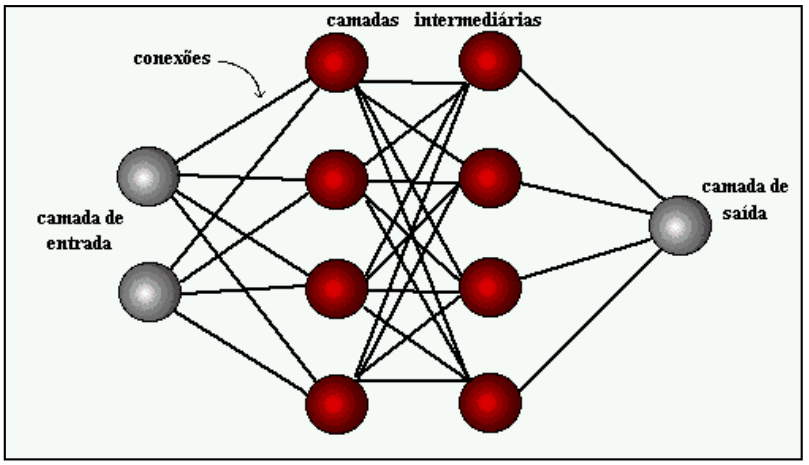
\includegraphics[scale=0.56]{Figuras/Redes_neural.png}
	\end{center}
    \legend{Fonte:\cite{Cortes2002}}
\end{figure}

\par
Segundo \citeonline{Cortes2002}, apresentado na Figura 8, todas as camadas intermediárias simbolizam os diferentes níveis de conhecimento que são obtidos no processo de seu percurso, numa tentativa de copiar o cérebro humano. Apesar de ser uma técnica poderosa, redes neurais é pouco utilizado em mineração de dados, pelo fato de seus algoritmos serem em sua maioria, incompreensíveis e também a função de aprendizado ser consideravelmente lenta, devido as várias interações que o algoritmo de retropropagação realiza para atualizar os valores da rede \cite{Carvalho2014}. 



\subsubsection{\textit{Support Vector Machines} (SVM)}

\par
Máquina de vetores de suporte é um algoritmo supervisionado que é usado para o trabalho de classificação, onde ele utiliza um hiperplano como separador de classes. Este hiperplano é encontrado através da utilização do conjunto de treinamento (vetores de suporte) e ele trabalha como uma base para o limite da decisão ao classificar \cite{Costa2012}. Segundo \citeonline{Henke2011}, ela é uma técnica de classificação bastante aplicada em problemas de segurança, como por exemplo na detecção de \textit{phishing} e detecção de intrusos.

\par
O funcionamento do SVM pode ser dito da seguinte forma: se tem duas classes e um conjunto de treinamento onde as amostras pertencem as classes, a máquina vetor de suporte cria um hiperplano (conhecido como hiperplano de separação ótima) que divide o espaço de atributos em duas regiões, potencializando a margem de separação entre as mesmas. As amostras que antes não eram conhecidas são mapeadas para esse mesmo espaço e depois atribuídas a uma das classes \cite{Henke2011}.

\begin{figure}[!htp]
	\begin{center}
    \caption{\label{fig:waveform_fig} Dados de treinamentos representando alunos que passaram (círculos brancos) e não passaram (círculos cinzas) em uma disciplina.}
	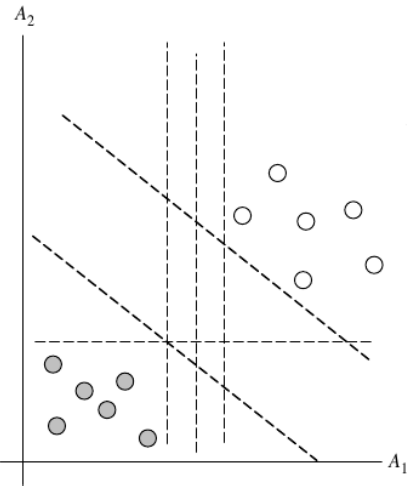
\includegraphics[scale=0.60]{Figuras/SVM.png}
	\end{center}
    \legend{Fonte:\cite{Costa2012}}
\end{figure}

\par
Como exemplo acima na Figura 9, suponhamos que os dados de treinamento sejam referentes aos alunos de uma turma com suas informações, apresentados como círculos, como a quantidade de postagens em um fórum de discussão (variável preditora). Além que, os dados representam cada aluno conforme o seu desempenho na disciplina (variável preditiva), alunos que passaram (círculos brancos) e que reprovaram (círculos cinzas). A priori, a meta do SVM é encontrar a melhor maneira de separar os dois grupos de alunos \cite{Costa2012}.



\par
Pode-se notar que existe uma quantidade infinita de hiperplanos que são representas na Figura 9 como essas linhas tracejadas, que podem separar as classes demonstradas que no caso são os círculos brancos e círculos cinzas. Então o propósito da máquina vetor de suporte é de encontrar o melhor hiperplano que maximize a distância entre elas das classes vizinhas. Um exemplo do melhor hiperplano para os dados que foram mostrado na Figura 9 encontrado pelo SVM é apresentado na Figura 10 \cite{Costa2012}. 


\begin{figure}[!htp]
	\begin{center}
    \caption{\label{fig:waveform_fig} Representação do melhor hiperplano que separa as classe, encontrado pelo algoritmo de SVM.}
	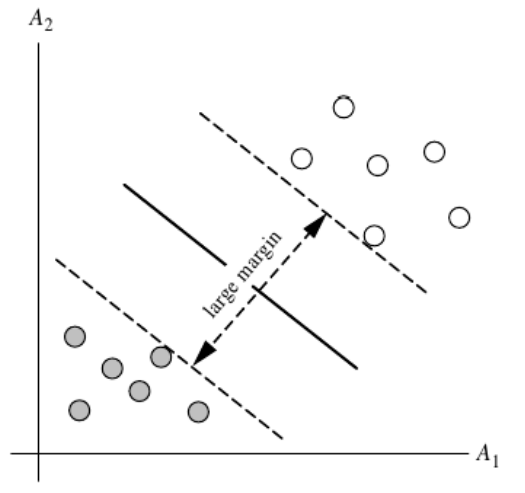
\includegraphics[scale=0.60]{Figuras/SVM_2.png}
	\end{center}
    \legend{Fonte:\cite{Costa2012}}
\end{figure}


\par
Embora SVM seja uma técnica recente, ela tem atraído muita atenção pelos seus resultados como: a possibilidade de modelar casos não-lineares difíceis gerando modelos de simples compreensão, consegue altos índices de assertividade, pode ser usada tanto para relações lineares quanto relações não lineares e entre outros \cite{Camilo2009}. Ultimamente um dos problemas dessa técnica é o tempo que se usa no aprendizado e muitas pesquisas estão se concentrando neste aspecto. 




%==========================
% MINERAÇÃO DE DADOS EDUCACIONAIS
%==========================

\section{Mineração de Dados Educacionais}

\par
Há pouco tempo, com o crescimento dos cursos a distância e também com aqueles que usam suporte computacional, muitos cientistas da área de Informática na Educação, têm demonstrado interesse em usar a mineração de dados para solucionar perguntas científica na área da educação \cite{Baker2011}. Nesse contexto, uma nova área de pesquisa surgiu denominada como Mineração de Dados Educacionais (MDE).

\par
A área de MDE (do inglês, \textit{Educational Data Mining}, EDM), é uma área que tem como proposito de desenvolver ou adaptar técnicas e algoritmos de mineração de dados existentes na literatura, de tal modo que sirvam a entender melhor os dados educacionais, gerados principalmente por professores e estudantes, tais como AVAs (Ambiente Virtual de Aprendizagem), STIs (Sistemas de Tutores Inteligentes), entre outros \cite{Costa2012, Marques2014}.

\par
Segundo \citeonline{Coutinho2016}, a MDE tem como apoio de disponibilizar a descoberta de conhecimentos que sejam importantes, único e útil, tais como: identificar padrões entre alunos, analisar o desempenho através de predição e a identificar perfis de forma que auxilie a gestão qualitativa da EAD. Os trabalhos nessa área, estão bastante concentrados em situações relacionados a um tipo específico de instituição, no caso, as Instituições de Ensino Superior (IES).

\par

